% Prevalence figure (preliminary, n=102 distinct JWT-validating configs).
% Real values with Wilson 95% CIs (asymmetric). Requires pgfplots in the preamble
% (the wrappers add it). \input this inside the Results section.
\begin{figure}[t]
\centering
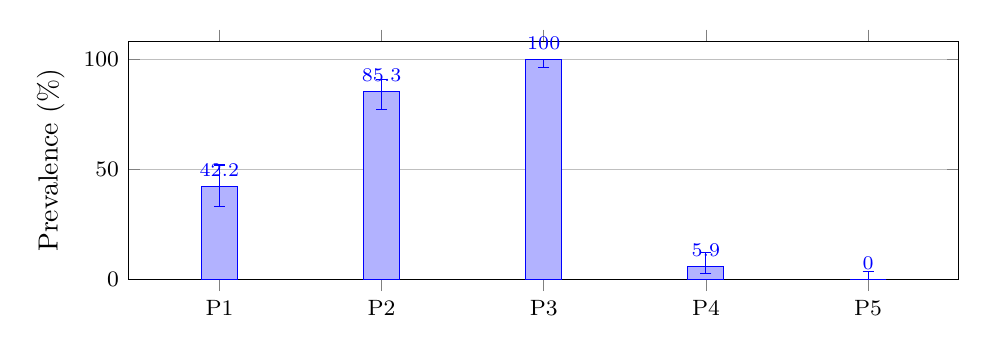
\begin{tikzpicture}
\begin{axis}[
  ybar, bar width=13pt,
  width=\linewidth, height=4.6cm,
  ymin=0, ymax=108, ylabel={Prevalence (\%)},
  symbolic x coords={P1,P2,P3,P4,P5},
  xtick=data, enlarge x limits=0.14,
  nodes near coords, nodes near coords align={vertical},
  every node near coord/.append style={font=\scriptsize},
  ymajorgrids, tick label style={font=\footnotesize},
]
% asymmetric explicit errors:  += (0, upper)  -= (0, lower)
\addplot+[error bars/.cd, y dir=both, y explicit]
coordinates {
  (P1,42.2)  += (0,9.7)  -= (0,9.2)
  (P2,85.3)  += (0,5.6)  -= (0,8.2)
  (P3,100.0) += (0,0.0)  -= (0,3.6)
  (P4,5.9)   += (0,6.3)  -= (0,3.2)
  (P5,0.0)   += (0,3.6)  -= (0,0.0)
};
\end{axis}
\end{tikzpicture}
\caption{Prevalence of cited verification weaknesses across 102 distinct
JWT-validating configurations, with Wilson 95\% confidence intervals.
P1 unbound audience; P2 no required claims; P3 no algorithm pinning \emph{in
configuration} (library-default caveat, \S\ref{sec:results}); P4 multi-issuer
(descriptive); P5 clock skew $>5$\,min. \textbf{Preliminary} (small $N$, no human
labels); see \S\ref{sec:limitations}.}
\label{fig:prevalence}
\end{figure}